%!TEX root = latex.tex

\begin{frame}[fragile]{Summary}
  \begin{enumerate}
    \item The \alert{\LaTeX-File} contains \alert{content and structure}.
    \item \LaTeX\ typesets a \alert{PDF-document} and ensures proper \alert{form}.
    \item Creating {new Layouts} is advanced.
    \item A \LaTeX-document contains the \alert{document class}, \alert{preamble} und \alert{document body}.
    \item \LaTeX\ is very useful for \alert{longer Documents} as it provides many possibilities for \alert{structuring} and
      \alert{outlining}. A document can be build from
      \alert{many source files}.
    \item \alert{\BibTeX} generates a \alert{bibliography} from a \alert{data base} in a special format. There are many \alert{bibliography styles} to choose from via \lstinline-\bibliographystyle-.
  \end{enumerate}
\end{frame}

\begin{frame}{The \LaTeX-Textbook}
  \begin{center}
    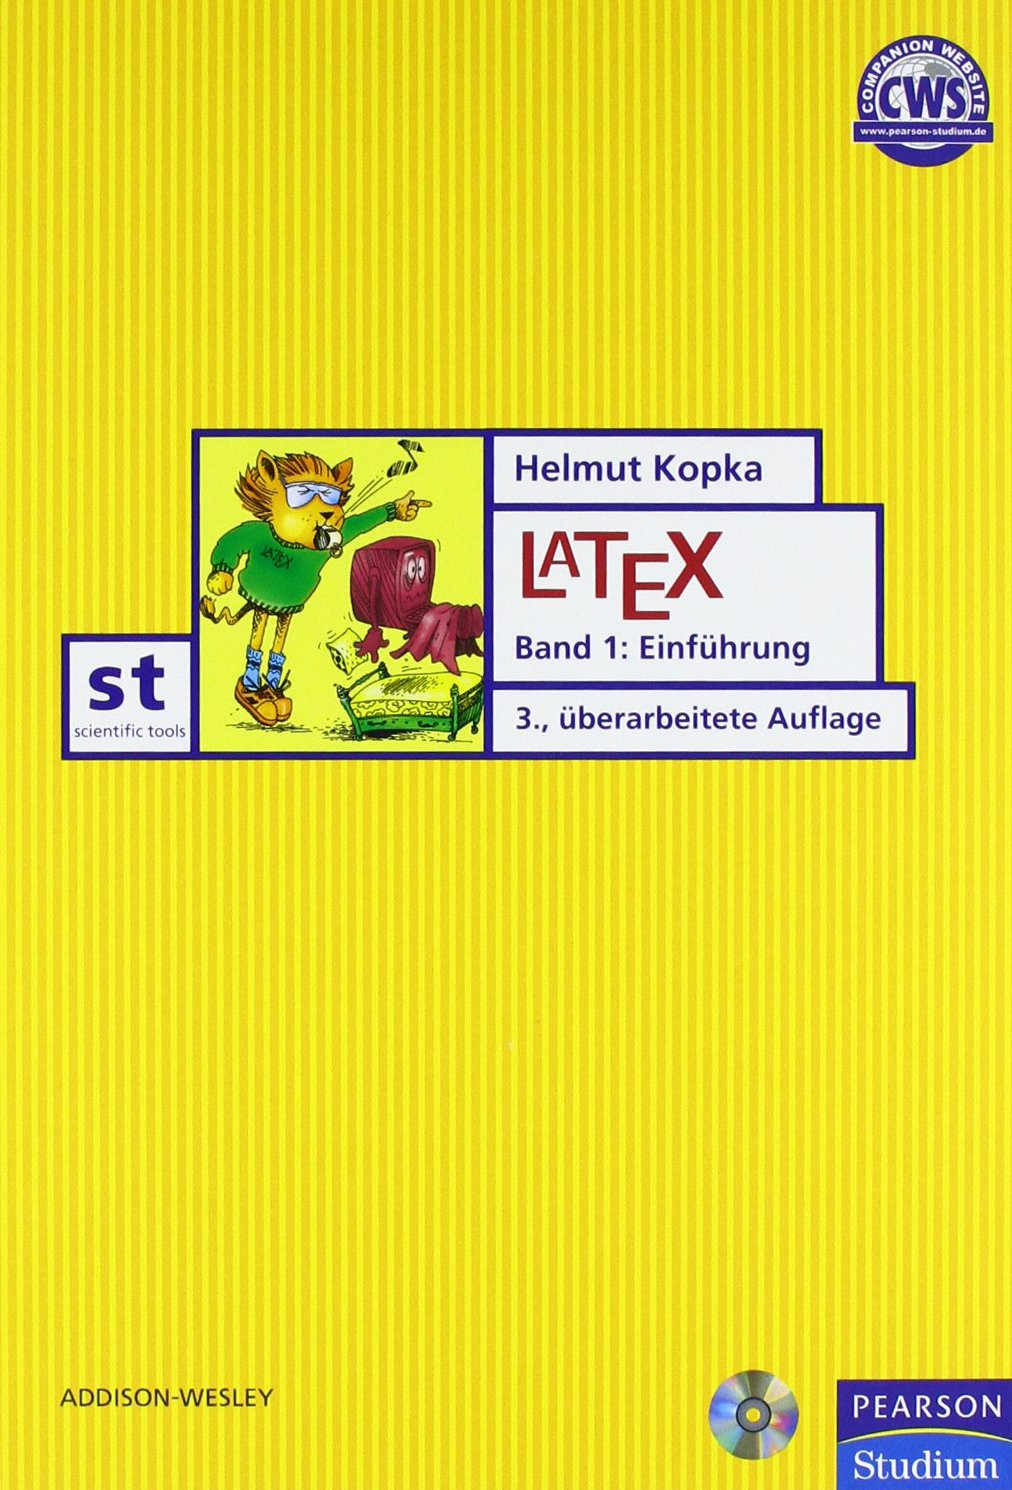
\includegraphics[width=5cm]{buecher/kopka}
  \end{center}
\end{frame}

\begin{frame}{Modern \LaTeX-Introduction}
  \begin{center}
    
\includegraphics[width=5cm]{buecher/schlosser}
  \end{center}
\end{frame}

\begin{frame}{Online \LaTeX-Referenz}
  \begin{center}
    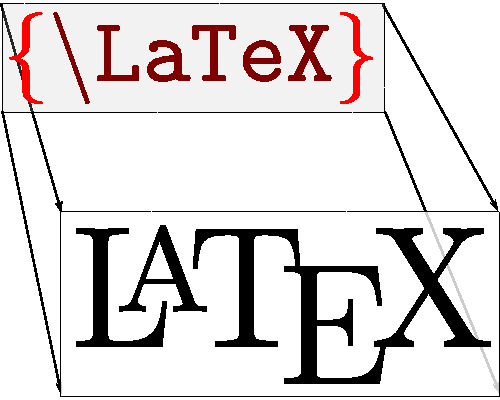
\includegraphics[width=5cm]{buecher/wikibook}

    \xxx

    \Huge Wikibook
  \end{center}
\end{frame}

